\subsection{Visualizing alignments with \sft{esl-ssudraw}}

SSU rRNA alignments are large and difficult to view in a meaningful
way. The \prog{esl-ssudraw} program introduced for visualizing masks
earlier in this tutorial can be also used to display statistics of
a particular alignment on the consensus SSU secondary structure of the
model used to create the alignment. As before,
using \prog{esl-ssudraw} requires a template postscript file of the
consensus secondary structure. The template files for the 3 default
\textsc{ssu-align} version 0.1 seed models are included as
\prog{\$INFDIR/ssu-align-0.1/seeds/ss-diagrams/{archaea,bacteria,eukarya}-0p1.ps}. 
(Unfortunately, it is difficult to create new template files for
additional models you might build for your own analyses.) 

\prog{esl-ssudraw} can be run in two different modes. In the default
mode, \emph{alignment} mode, the structure diagrams will display
statistics on the alignment. In \emph{individual} mode, the structure
diagrams will show individual sequences in the alignment by displaying
the actual residues at each consensus position of the alignment. Note
that the diagrams are always of the consensus model defined in the
template file. In alignment mode, only statistics of consensus
positions are displayed. In individual mode, only residues that align to
consensus positions are displayed.

The following table summarizes the different statistics that can be
created in alignment mode.
An example of each of these types of
diagrams is included as the indicated figure for the default
eukaryotic seed alignment. The postscript and pdf files for each of
these included figures, as well as analogous diagrams for the
archaeal and bacterial seeds are included in 
\prog{\$INFDIR/ssu-align-0.1/seeds/ss-diagrams/}, named as indicated 
in the ``file'' column of the table. 

\begin{center}
\begin{tabular}{llll} \hline
\prog{esl-ssudraw} option(s) & statistic                     &  figure & file \\ \hline
\prog{<none>}                & information content           & \ref{fig:eukinfo} & \prog{eukarya-0p1-info} \\
& & & \\
\prog{-q --prob}                & average posterior probability & \ref{fig:eukprob} & \prog{eukarya-0p1-prob} \\
& & & \\
\prog{-q --ins}                 & frequency of insertions       & \ref{fig:eukins}   & \prog{eukarya-0p1-ins} \\
                             & after each position           & & \\
& & & \\
\prog{-q --dall}                & frequency of deletions        & \ref{fig:eukdall}  & \prog{eukarya-0p1-dall} \\
& & & \\
\prog{-q --dint}                & frequency of internal deletions & \ref{fig:eukdint}  & \prog{eukarya-0p1-dint} \\
                             & (excluding terminal deletions)  & & \\
& & & \\
\prog{-q --struct}              & additional information from     & \ref{fig:eukstruct} & \prog{eukarya-0p1-struct} \\
                             & conserved structure \\
\end{tabular}
\end{center}

If more than one of these options are used, the program will create a
multi-page postscript document with each diagram on a separate page.
If the \prog{-q} option is omitted, the program will create the
information content diagram as the first page by default.
As an example of how these files were created, the command

\user{esl-ssudraw -q --dall ../eukarya-0p1.stk eukarya-0p1.ps eukarya-0p1-dall.ps}

was used to create Figure~\ref{fig:eukdall} while in the 
\prog{\$INFDIR/ssu-align-0.1/seeds/ss-diagrams/} directory.

\newpage

\begin{figure}
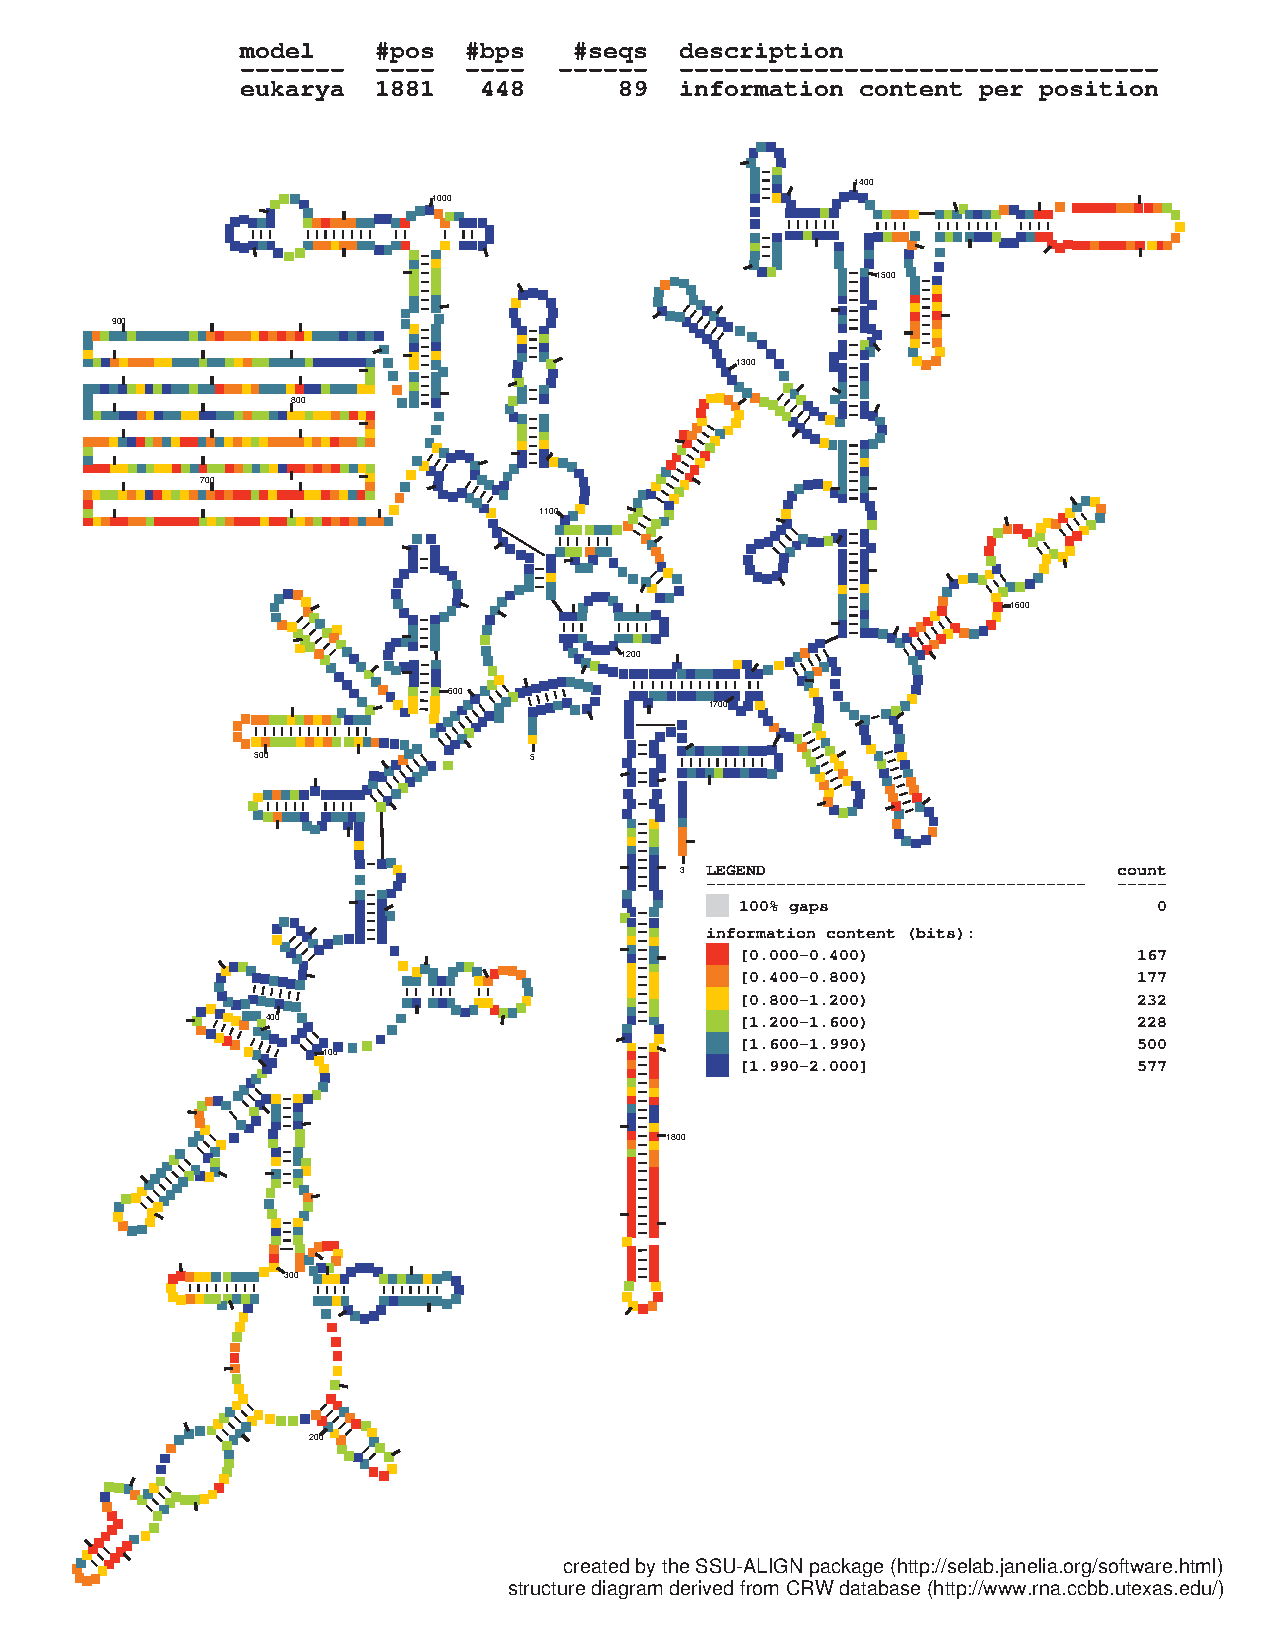
\includegraphics[height=8.5in]{Figures/eukarya-0p1-info}
\label{fig:eukinfo}
\end{figure}

\newpage

\begin{figure}
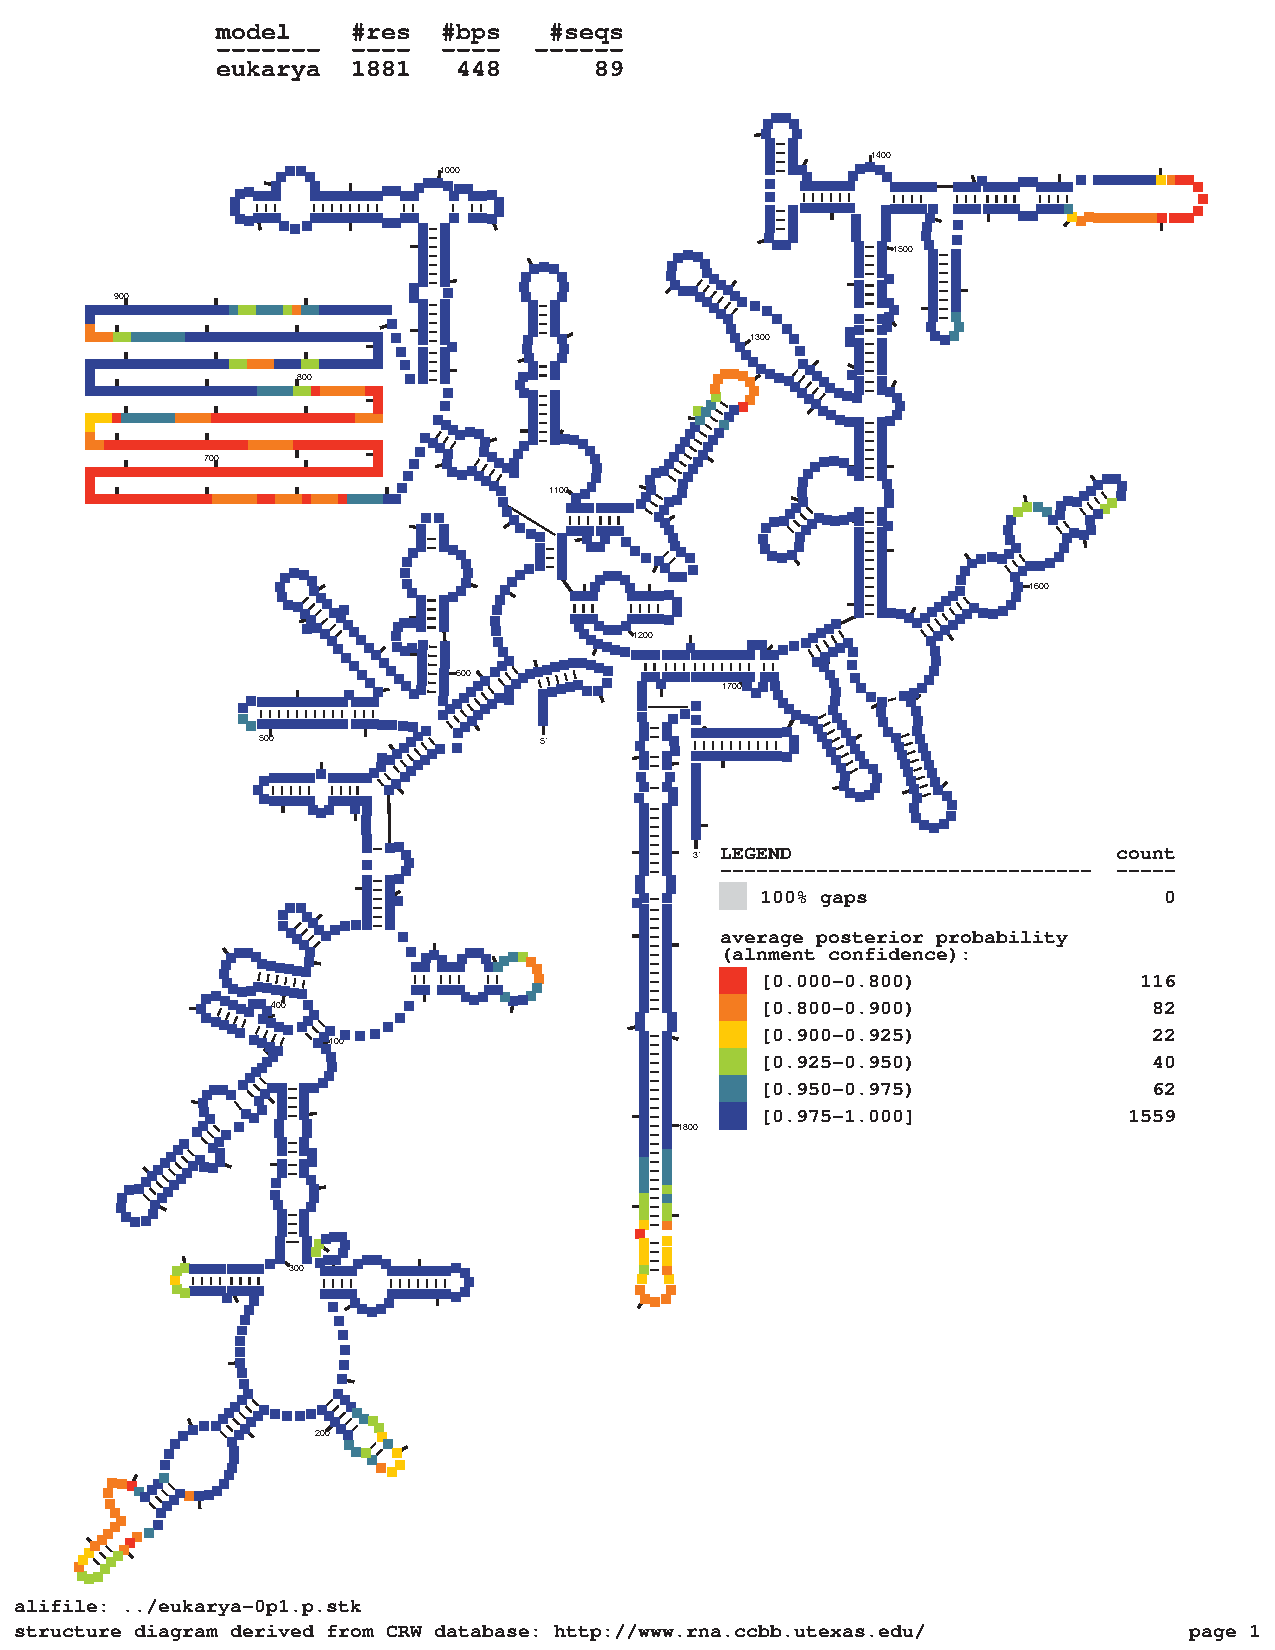
\includegraphics[height=8.5in]{Figures/eukarya-0p1-prob}
\label{fig:eukinfo}
\end{figure}

\newpage

\begin{figure}

\includegraphics[height=8.5in]{Figures/eukarya-0p1-ins}
\label{fig:eukinfo}
\end{figure}

\newpage

\begin{figure}
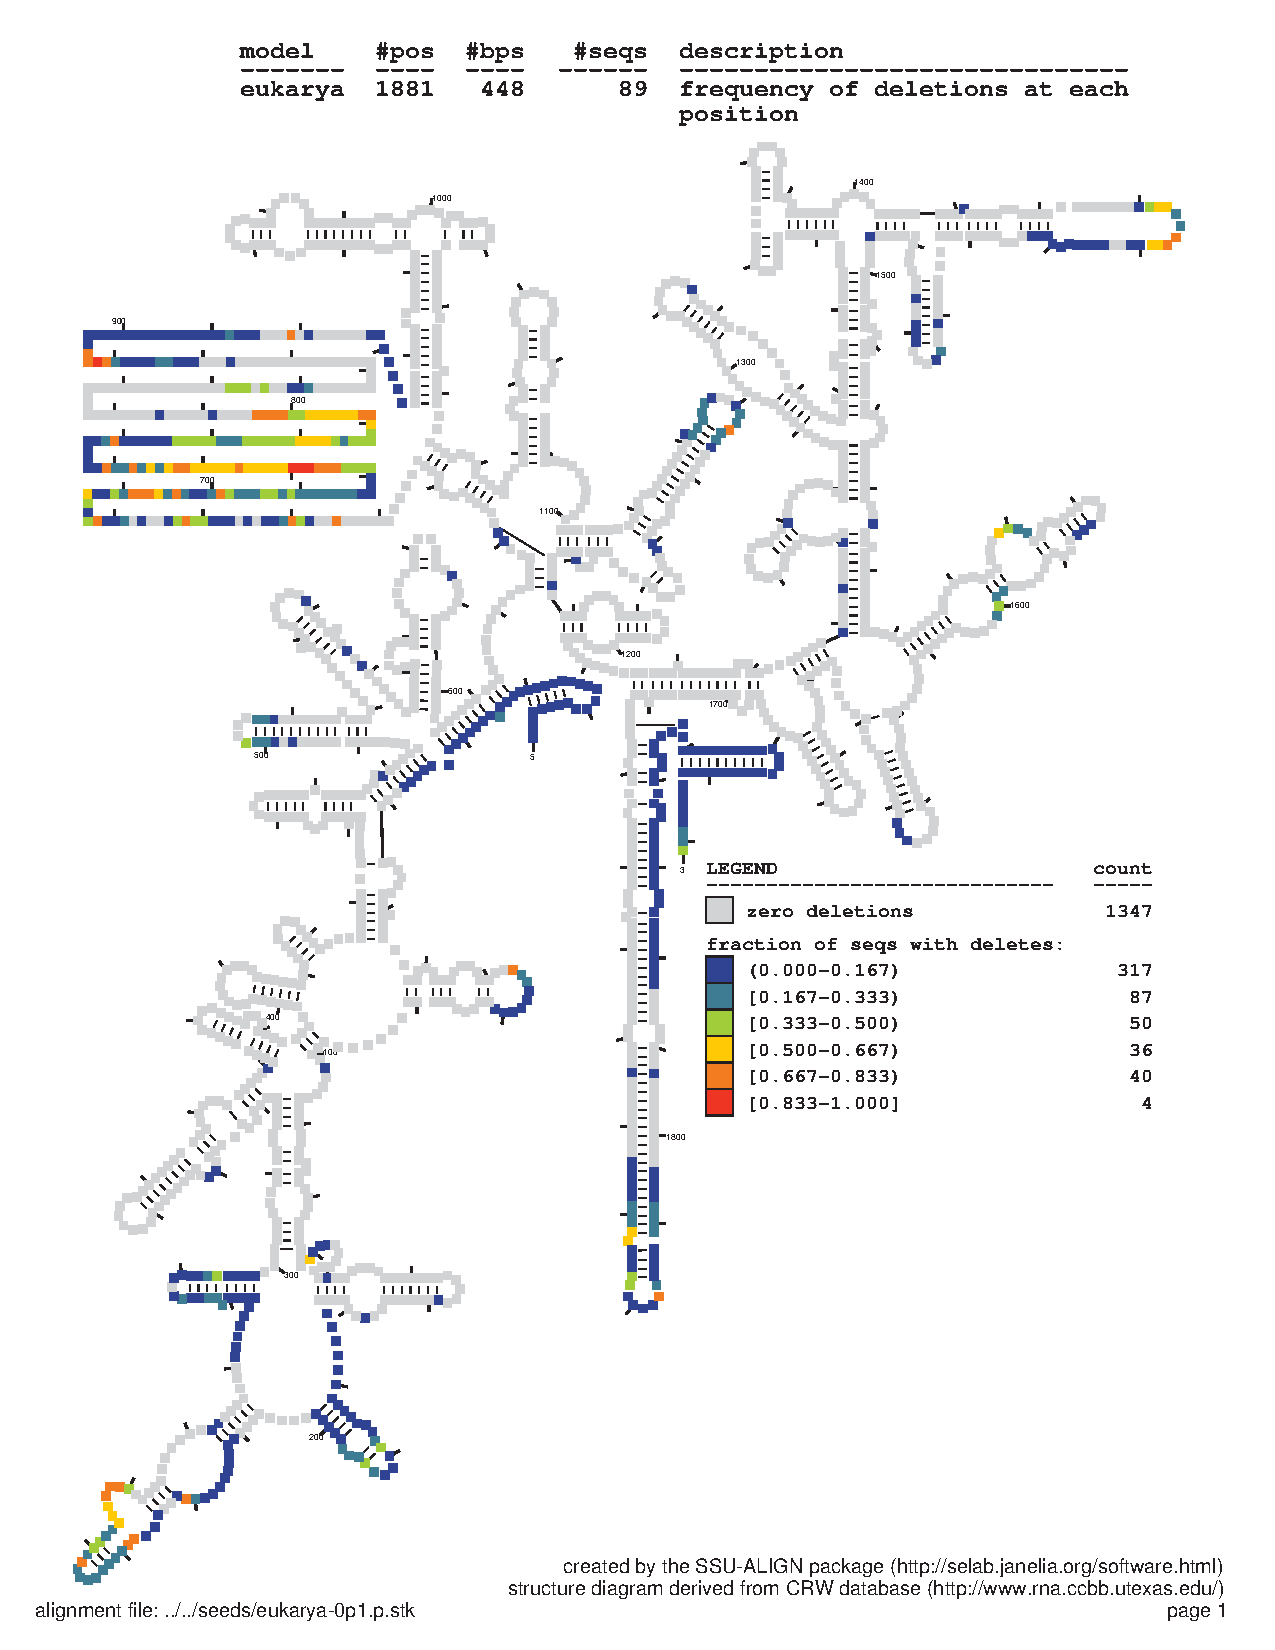
\includegraphics[height=8.5in]{Figures/eukarya-0p1-dall}
\label{fig:eukinfo}
\end{figure}

\newpage

\begin{figure}
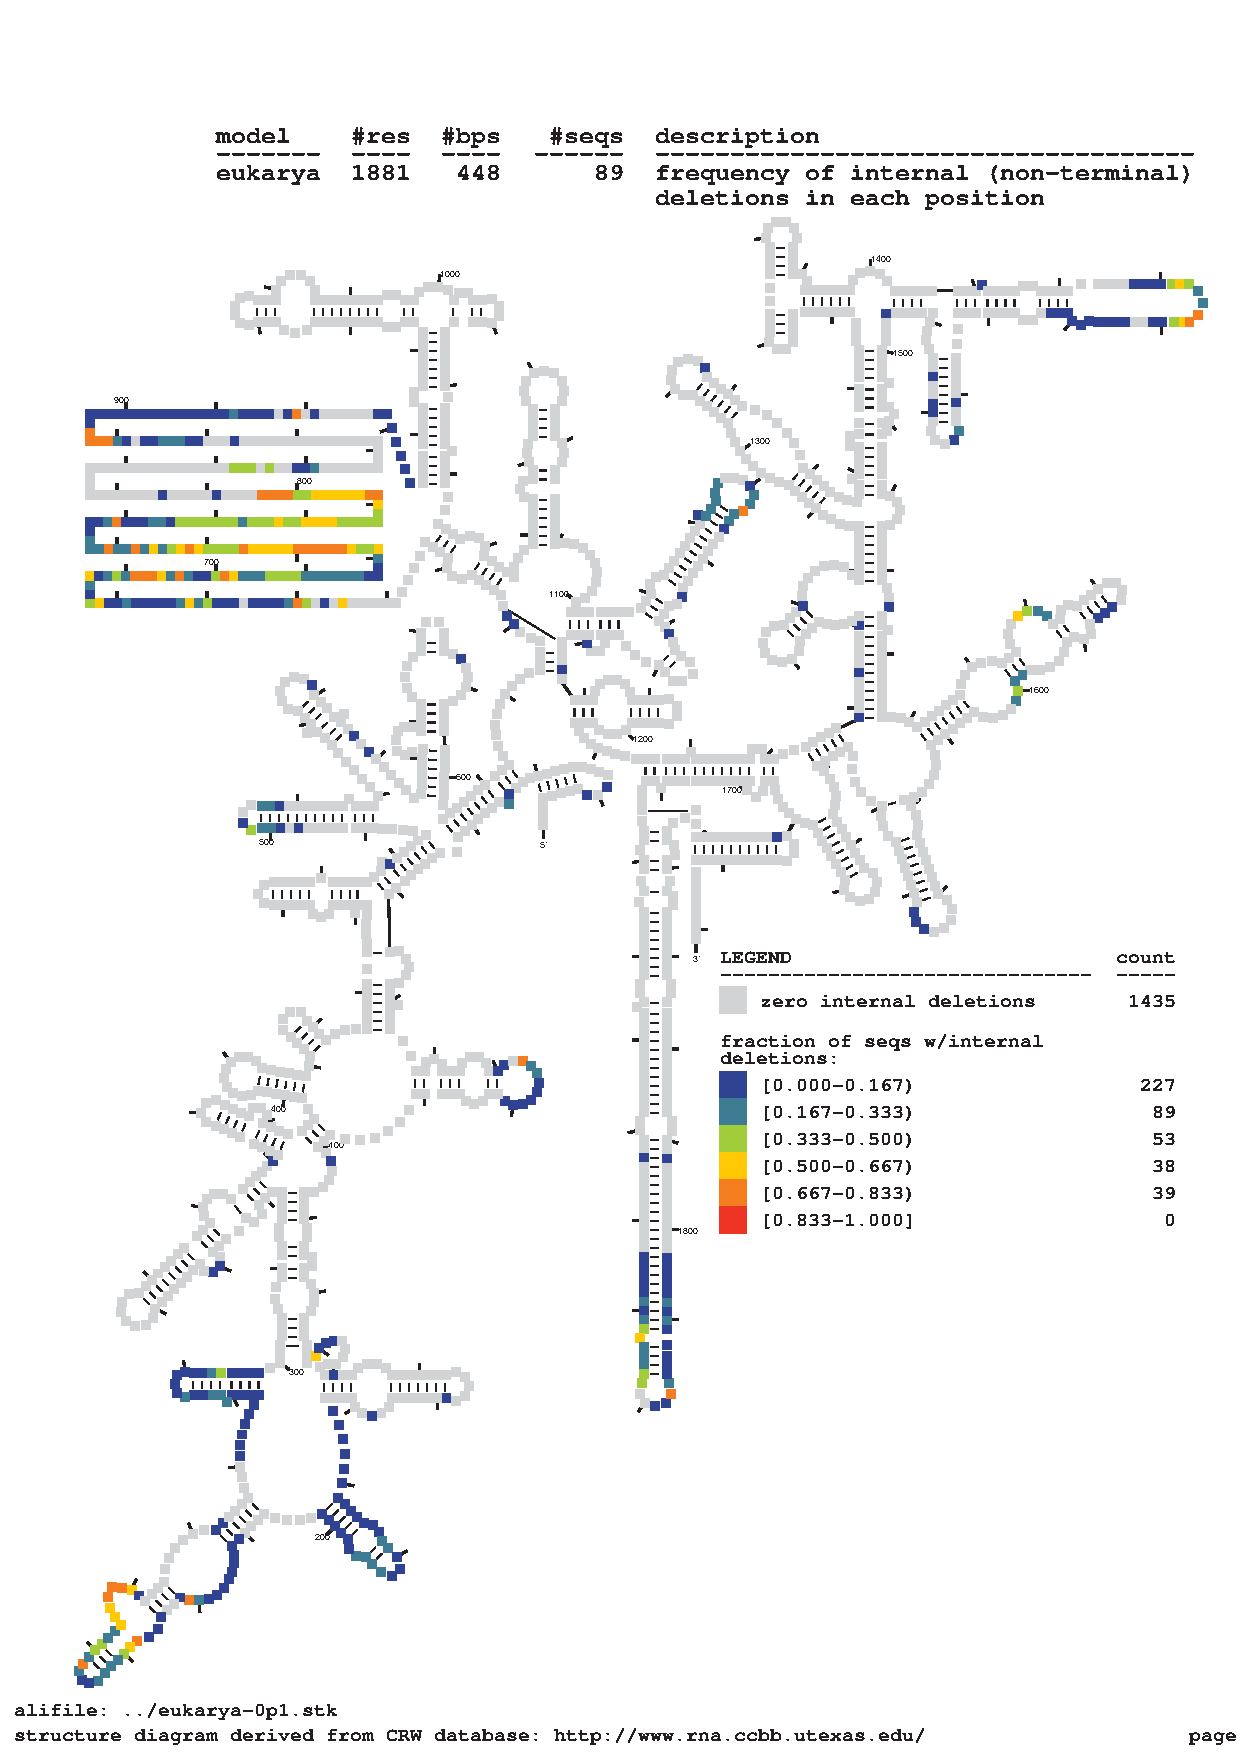
\includegraphics[height=8.5in]{Figures/eukarya-0p1-dint}
\label{fig:eukinfo}
\end{figure}

\newpage

\begin{figure}
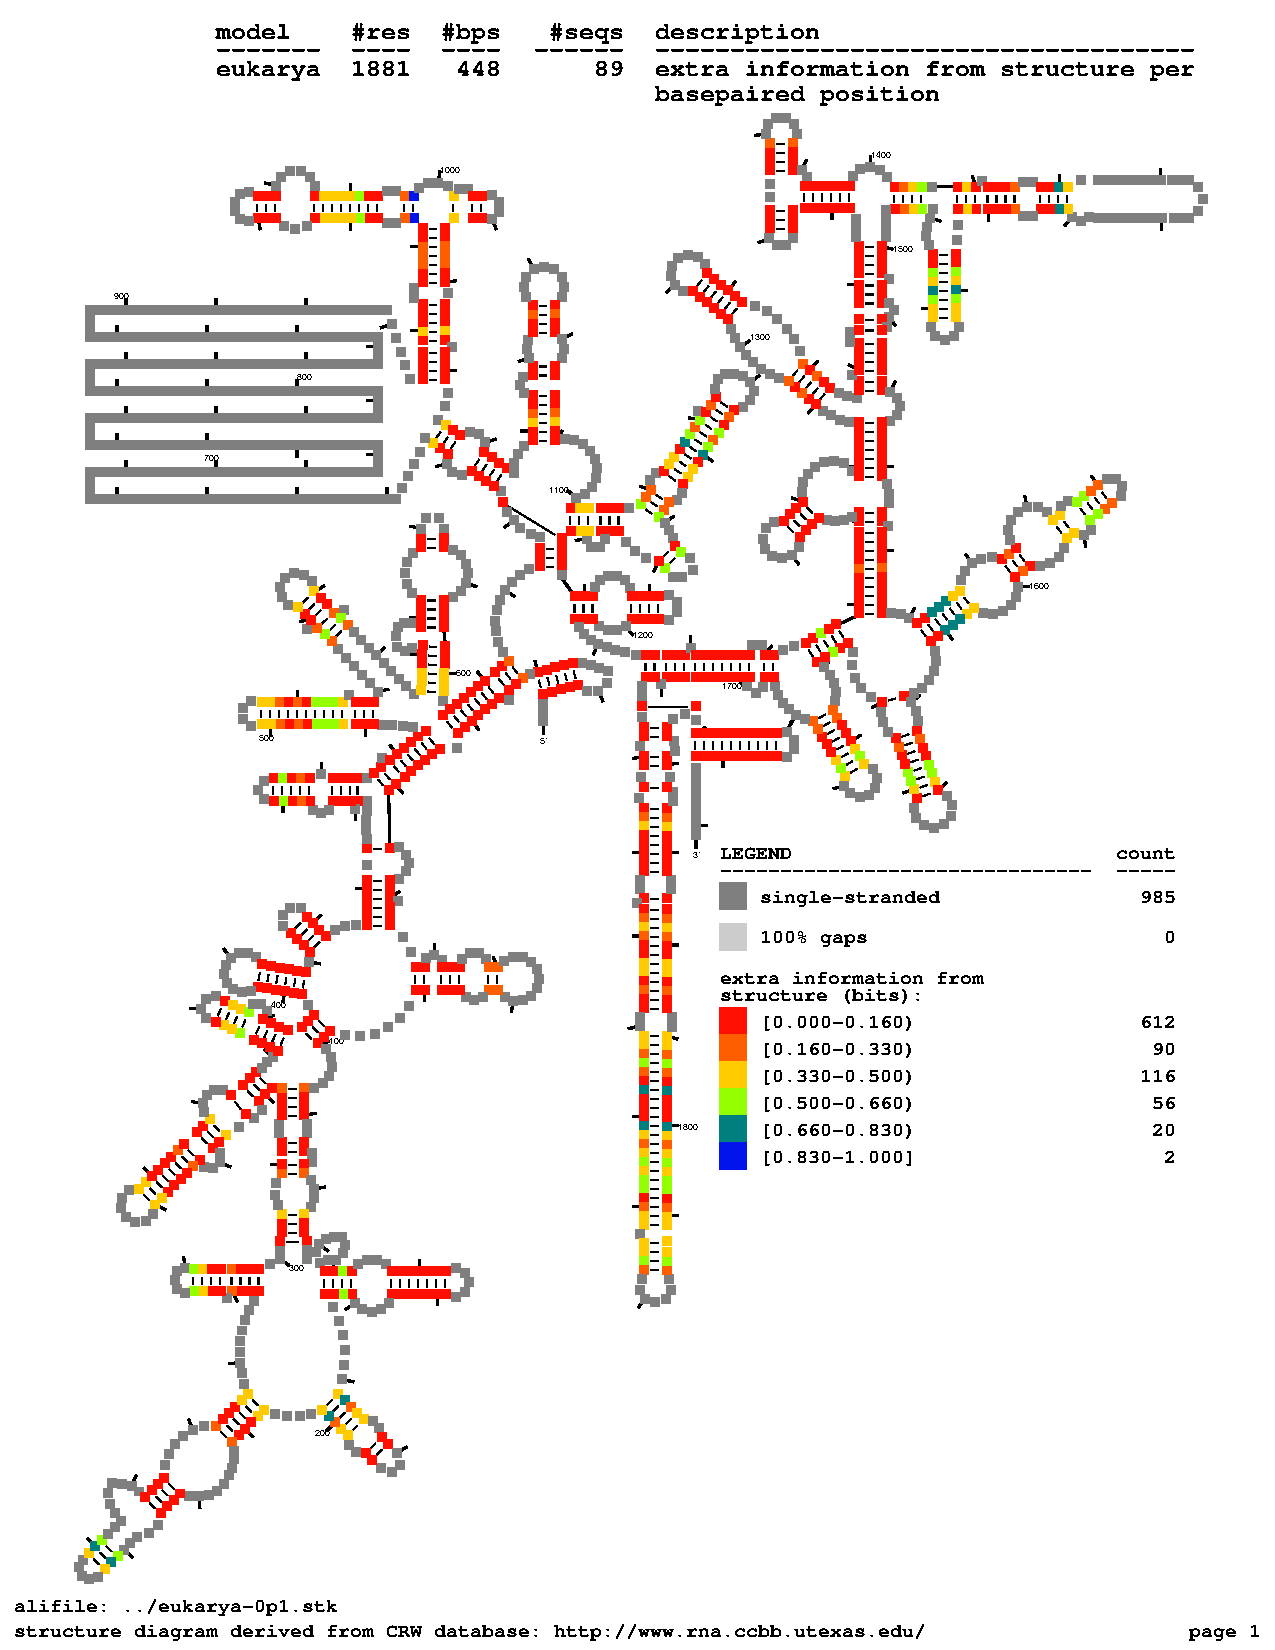
\includegraphics[height=8.5in]{Figures/eukarya-0p1-struct}
\label{fig:eukinfo}
\end{figure}






